\documentclass[12pt, titlepage]{article}

%% Comments
\newif\ifcomments\commentstrue

\ifcomments
\newcommand{\authornote}[3]{\textcolor{#1}{[#3 ---#2]}}
\newcommand{\todo}[1]{\textcolor{red}{[TODO: #1]}}
\else
\newcommand{\authornote}[3]{}
\newcommand{\todo}[1]{}
\fi

\newcommand{\wss}[1]{\authornote{magenta}{SS}{#1}}
\newcommand{\ds}[1]{\authornote{blue}{DS}{#1}}

%% Graphics
\usepackage{graphicx}
\graphicspath{ {Images/} }

\begin{document}

\title{Smart Waiter Software Requirements} 
\author{Meraj Patel (1137491)\\ Pavneet Jaual ()\\ Shan Perera ()}
\date{\today}
\maketitle

\tableofcontents 
\listoffigures
\listoftables

\section*{Revision History}
\begin{tabular}{|c|c|}
\hline
\textbf{Date}  & \textbf{Comments} \\ \hline
October 9, 2015 & Created first draft. \\ 
\hline
\end{tabular}

\section*{Template}
This document makes use of the Volere Template for all of its organization.


\section{Project Drivers}

\subsection{The Purpose of the Project}
This project aims to provide a solution that will allow users to order and pay through a mobile application at restaurants. This opportunity arose from the lack of a universal application in the market, which allows users to visit multiple restaurants, and order and pay at each restaurant, through the singular application. Once complete, the Android users will be able to walk into any restaurant which offers our solution, and have the ability to order and pay for their meal through the singular application.
\subsubsection{Project Goal}
The delivered application will allow an Android user to use the application at any restaurant, which offers the Smart Waiter solution.  More importantly, the client should be able to view restaurants complete menu, order selected items and pay for their meal through the application. 
\subsection{The Client, the Customer, and Other Stakeholders}
\subsubsection{The client}
The prospective client of this application will be a restaurant owner or manager, who would like to implement an application based ordering system at their restaurant.
\newline
\newline
\subsubsection{The Customers}
The targeted customers will include clients of the restaurants, which offer Smart Waiter solution.
\newline
\newline
\subsubsection{Other Stakeholders}
Other Stakeholders of this project include:
\begin{itemize}
  \item Supervisor – Dr. Rong Zheng
  \item 	Android Users – Clients of restaurant
  \item 	Developers and Testers – Pavneet Jaual, Meraj Patel and Shan Perera
  \item 	Beta Testers
  \item Prospective manager/restaurant owners \ldots
\end{itemize}

\subsection{Users of the Product}
\subsubsection{The Hands-On Users of the Product}

\textbf{\textit{Group - Restaurant clients}}\newline
Clients who frequent restaurants, which offer Smart Waiter services.\newline
\newline
\textit{User Role}\newline
These users will use the application to view restaurant menu, order their selection and pay for their meal.\newline\newline
\textit{Subject Matter Experience}\newline
These users can be categorized as novice, as they do not need extensive knowledge of the business. The user can simply be a client walking into a restaurant for the first time.\newline\newline
\textit{Technological Experience}\newline
The technological experience of this user can also be considered novice. The application will not require any training to use.\newline\newline
\textit{Other User Characteristics}\newline
There are some basic characteristics that the user should have, to qualify to use this application:
\begin{itemize}
  \item Should have an android device and an internet connection
  \item Basic understanding of how to use an android application. 
  \item 	Should have a credit card, to make payments through the application. 
  \item 	Users who generally frequent restaurants at least once a month
\end{itemize}

\textbf{\textit{Group - Restaurant Owners}}\newline
Restaurant managers who have Smart Waiter solutions implemented \newline
\newline
\textit{User Role}\newline
These users will use the application to view restaurant menu, order their selection and pay for their meal.\newline\newline
\textit{Subject Matter Experience}\newline
To be considered masters, as they have in depth knowledge of the business. \newline\newline
\textit{Technological Experience}\newline
The technological experience of this user can be considered novice. The application will not require any training to use. \newline\newline
\textit{Other User Characteristics}\newline
There are some basic characteristics that the user should have, to qualify to use this application;
\begin{itemize}
  \item Should have an android device and an internet connection
  \item Basic understanding of how to use an android application. 
  \item 	Credit card required if they want to test payments method 
  \item 	These users will pay attention to details. They will generally critique the UI and other aspects of the application to see how it fits their specific business needs.
\end{itemize}

\textbf{\textit{Group – Testers/Developers}}\newline
Testers and developers of Smart Waiter \newline
\newline
\textit{User Role}\newline
These users will perform end-to-to system testing. The tester and developers will verify that each use-case and each feature in the application works correctly. \newline\newline
\textit{Subject Matter Experience}\newline
They will have complete knowledge of the business needs and requirements. Thus they can be considered a master. \newline\newline
\textit{Technological Experience}\newline
They will be a master in technological experience. They will know the code base of the application thoroughly. Similarly, they would know the application infrastructure and other technology used in the application. \newline\newline
\textit{Other User Characteristics}
\begin{itemize}
  \item Advanced knowledge of android framework
  \item Advanced knowledge of the code base
  \item 	Evaluate the application from the engineering perspective
  \item 	These users will pay close attention to detail
  \item 	Knowledge of all possible use-cases and expected outcomes of the application
\end{itemize}

\subsubsection{Priority assigned to the user}
\textit{Key Users }\newline
The key users of this application will be the target market of this product. Namely, the restaurant owners/managers and the restaurant clients.\newline
\newline
\textit{Secondary Users}\newline
The secondary users will be considered the Testers/Developers.
\newline

\subsubsection{User Participation}
\textit{Restaurant Clients}\newline
These users will be participating and helping us provide the requirements and throughout the lifetime of the application. Specifically, they will be having a “report bug” feature built into the application to report bugs and suggest improvements. They will provide usability requirements.\newline
\newline
\textit{Restaurant Owners}\newline
These users will also participate in providing requirements throughout the lifetime of the application. However, their main concerns are expected within 1 day of application usage. These users will provide business knowledge and business requirements for the application.
\newline
\newline
\textit{Testers/Developers }\newline
Throughout the development cycle of the application these users will continuously contribute to the requirements of the application. Specifically, they will provide interface prototyping, business knowledge and usability requirements for  the application.
\newline
\newline

\subsubsection{Maintenance Users}
The testers/ Developers of the application will be considered the maintenance users. When going through the steps of unit testing, end-to-end testing and verification process, these users will continuously make changes to improve the product.

\section{Project Constraints}
\subsection{Mandated Constraints}

\subsubsection{Solution Constraints}
\textbf{\textit{Constraint 1}}
\newline
\textit{Description}\newline
The application shall pull the restaurant’s menu from the server via a barcode scan.\newline\newline
\textit{Rationale}\newline
Provide a simple solution, which supports multiple restaurants. \newline\newline
\textit{Fit criterion}\newline
Must be approved by tester and developer. They must confirm that complete information about the restaurant’s menu has been pulled from the server onto the user’s device.\newline\newline

\textbf{\textit{Constraint 2}}
\newline
\textit{Description}\newline
The barcode scan by user shall send table and other user information to the server.\newline\newline
\textit{Rationale}\newline
Provide the restaurant with client’s information and table number to serve food too. \newline\newline
\textit{Fit criterion}\newline
Must be approved by tester and developer. They must confirm that complete information about the user has been pushed to the server onto the user’s device.\newline\newline

\textbf{\textit{Constraint 3}}
\newline
\textit{Description}\newline
The application must run on Android operating system. \newline\newline
\textit{Rationale}\newline
We are catering to the entire android platform users. \newline\newline
\textit{Fit criterion}\newline
The application must be approved complaint from the developers and testers. This will involve thorough testing on the Android platform.\newline\newline

\textbf{\textit{Constraint 4}}
\newline
\textit{Description}\newline
The application shall support credit card payments. \newline\newline
\textit{Rationale}\newline
This will transfer money to the restaurant account. \newline\newline
\textit{Fit criterion}\newline
The functionality must be approved complaint by the developer and testers. This will require approving the code base and the end-to-end functionality.\newline\newline

\textbf{\textit{Constraint 5}}
\newline
\textit{Description}\newline
The payment information for the client must be stored safely \newline\newline
\textit{Rationale}\newline
This is very sensitive data and should not be abused and exploited. \newline\newline
\textit{Fit criterion}\newline
The functionality must be approved complaint by the developer and testers. This will require approving the code base and the end-to-end functionality.\newline\newline

\subsubsection{Implementation Environment of the Current System}
The environment will require the following;
\begin{itemize}
  \item Source code will be written in Java
  \item Android Studio will be used as the IDE
  \item 	Parse API Library for Android will be used for cloud storage
  \item 	Stripe API will be used to process credit card payments
\end{itemize}

\subsubsection{Partner or collaborative applications}
Not Applicable \newline\newline

\subsubsection{Off-the-shelf software}
Sketch will be used to make UI blueprints. In addition, Photoshop will be used to make custom logos and icons. \newline\newline

\subsubsection{Anticipated workplace environment}
The users will be using this application in a restaurant. Typically, this work environment would be loud and distracting. Thus, we plan on making the UI of the application visually attractive, where the user does not need to read much.  \newline\newline

\subsubsection{How long will the developers have on the project}
The final deadline for the project is mid April 2016. The detailed deliverables and their respective deadlines are listed below;
\begin{itemize}
  \item Requirements Document Revision 0: October, 9, 2015 
  \item Proof of Concept Plan: October, 23, 2015
  \item 	Test Plan Revision 0: October, 30, 2015
  \item 	Proof of concept demonstration: November, 16, 2015  – November, 27, 2015
  \item Design document revision 0: January, 11, 2015
  \item Revision 0 Demonstration: February, 1, 2015  – February, 12, 2015
  \item User’s Guide Revision 0: February, 29, 2015
  \item 	Test Plan Revision 0: March, 21, 2015
  \item Final Demonstration: Mid-April, 2016
  \item 	Final Documentation for the product: April, 1, 2016
\end{itemize}


\subsection{Naming Conventions and Terminology}
N/A
\subsection{Relevant Facts and Assumptions} 
\subsubsection{Relevant Facts}
\textbf{\textit{Fact 1}}\newline
Stripe API used for payment processing is payment card industry (PCI) complaint.
\newline\newline
\textbf{\textit{Fact 2}}\newline
Restaurant clients should not be able to dine and dash.\newline

\subsubsection{Assumptions}

\textbf{\textit{Assumption  1}}\newline
Parse Database offers top-notch security for backend infrastructure from physical to application level.
\newline\newline
\textbf{\textit{Assumption  2}}\newline
SSL connection used for socket programming is secure and cannot be sniffed.

\section{Functional Requirements} 

\subsection{The Scope of the Work}
\subsubsection{The Current Situation}
An android application is required to allow customers to walk into a restaurant and use their smart device to view a menu, place an order and pay for there meal. This will be a singular solution extended to multiple restaurants so users only have to use one mobile application to serve these functions.   
\subsubsection{The Context of the Work} 
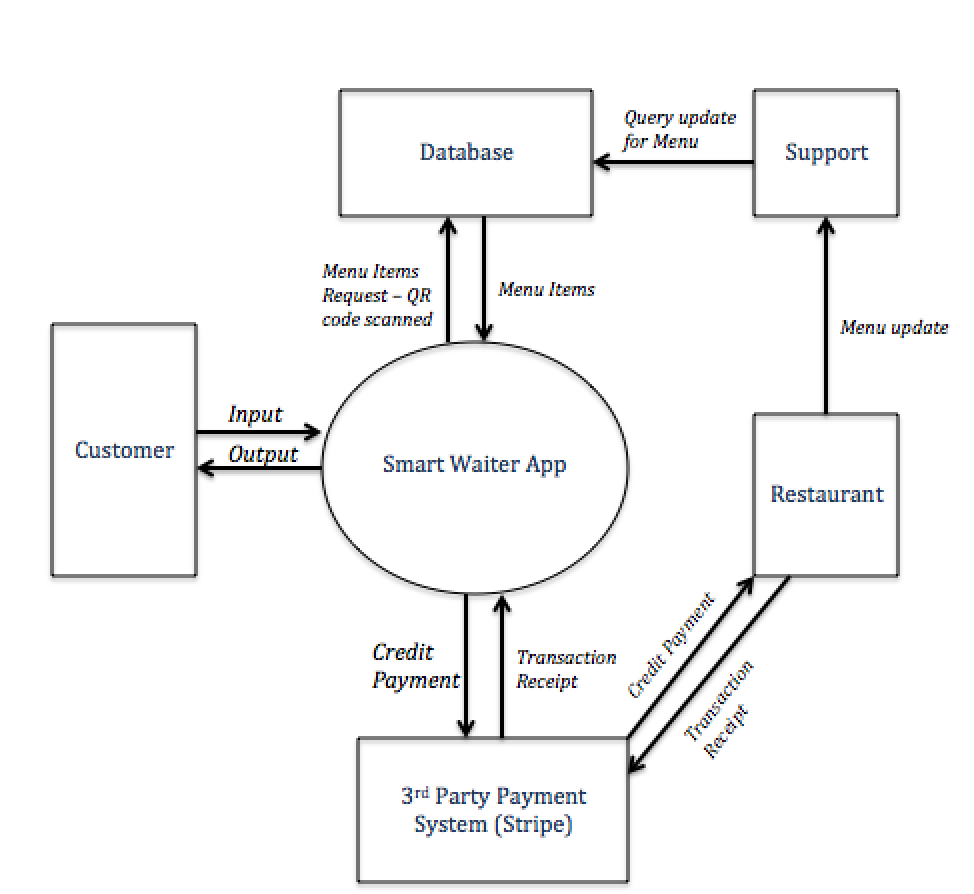
\includegraphics{Context.png}
\subsection{Business Data Model and Data Dictionary}
\subsubsection{Business Data Model}
\subsubsection{Data Dictionary}
\begin{center}
\begin{tabular}{ |c|c|c| }
\hline
Name & Content & Type \\
\hline
Restaurant & Restaurant Identifier & Class \\
User & User Identifier & Class \\
Waiter & Waiter Identifier & Class \\
Table & Table Identifier & Class \\
Order & Order Identifier & Class \\
Menu & Menu & Class \\
QR Code & QR Code & Class \\
User Identifier & Username + Password + Credit Card Info & Attribute/Element \\
Waiter Identifier & Employee Name + Employee Number & Attribute/Element \\
Table Identifier & Table Number + Waiter Assigned & Attribute/Element \\
Order Identifier & Table Number + User Identifier & Attribute/Element \\



\hline
\end{tabular}
\end{center}
\subsection{The Scope of the Product}
\subsubsection{Product Boundary}
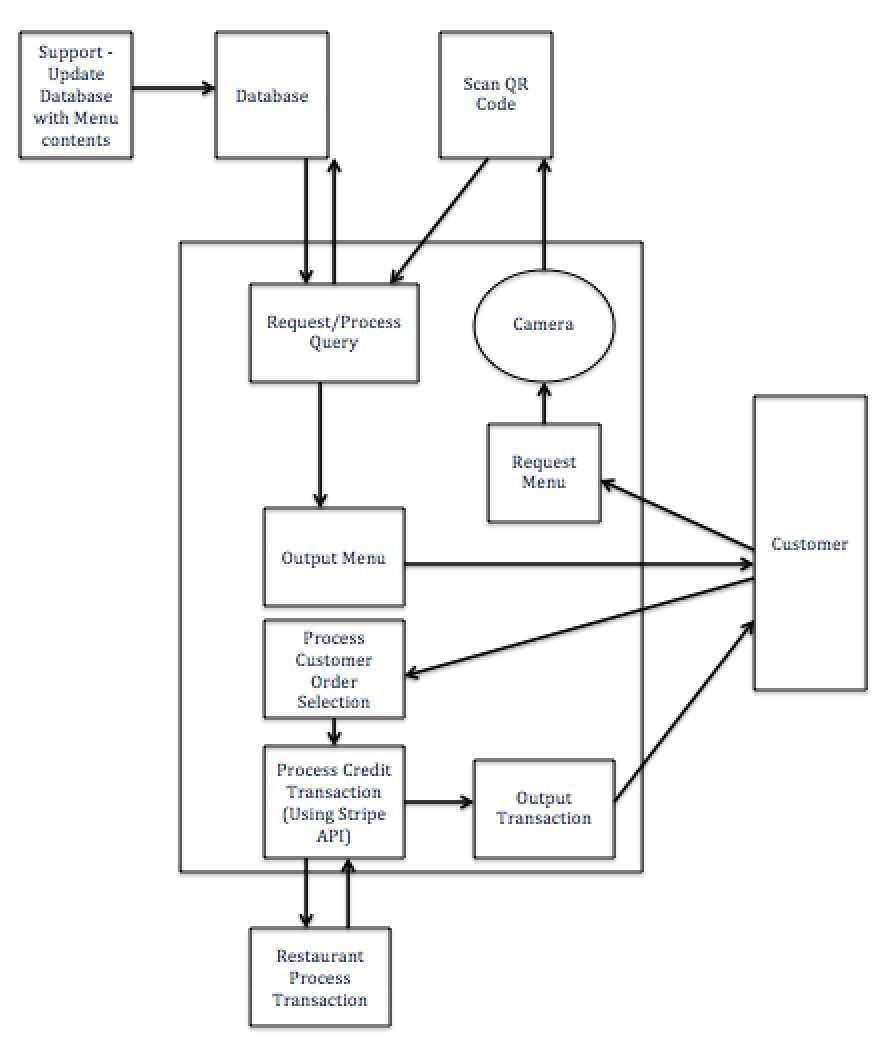
\includegraphics{ProductBoundary.png}
\subsubsection{Product Use Case Table}
\subsection{Functional Requirements}

\subsubsection{Functional Requirements}

\textbf{\textit{Requirement 1}}\newline
\textit{Description:}\newline
The product shall scan a QR code to access the restaurant's menu.\newline\newline
\textit{Fit Criterion:}\newline 
The product should access the camera application on the respective device to take a picture of the QR code and it will bring up the restaurant menu or display an error.
\newline

\textbf{\textit{Requirement 2}}\newline
\textit{Description:}\newline
The product shall allow the user to register an account for complete access to the products payment services. \newline\newline
\textit{Fit Criterion:}\newline 
The product will ask the user if they would like to register an account, if the user agrees: the product will bring them to the registration page asking the user to provide a username, password, and credit card information. If the user declines, the product will bring them back to the main menu of the application.
\newline

\textbf{\textit{Requirement 3}}\newline
\textit{Description:}\newline
The product will allow users to register using Google or Facebook accounts. \newline\newline
\textit{Fit Criterion:}\newline 
A user downloads the app and is asked to register an account, they decide they do not want to go through the trouble of creating a new account so they login with their Google account.
\newline

\textbf{\textit{Requirement 4}}\newline
\textit{Description:}\newline
The product shall allow the user to report bugs. \newline\newline
\textit{Fit Criterion:}\newline 
The product offers a menu to allow the user to report a bug they encountered. The user presses a button to report the bug and a pop-up form with a text entry box allows the user to describe the bug in 400 characters or less and sends the information to the developers through an automated email.
\newline

\textbf{\textit{Requirement 5}}\newline
\textit{Description:}\newline
The product shall provide error codes for common errors. \newline\newline
\textit{Fit Criterion:}\newline 
The user enters incorrect details when trying to login to their account. The product reports the error code 1, with the following message: Incorrect login information. i.e., Error Code 1: Incorrect login information.
\newline

\textbf{\textit{Requirement 6}}\newline
\textit{Description:}\newline
The product will display the menu in a similar fashion to the hard copy menu offered at the restaurant. \newline\newline
\textit{Fit Criterion:}\newline 
A user accesses the menu using the product, it looks similar, if not identical to the paper menu offered at the restaurant.
\newline

\textbf{\textit{Requirement 7}}\newline
\textit{Description:}\newline
The product will provide detailed information on a menu item when selected. \newline\newline
\textit{Fit Criterion:}\newline 
A user is browsing the menu and selects a hamburger, a new screen is brought up on the users device which details the ingredients of the hamburger and any extra ingredients they may add to the hamburger.
\newline

\textbf{\textit{Requirement 8}}\newline
\textit{Description:}\newline
The product will allow a user to request special instructions for food items they have ordered. \newline\newline
\textit{Fit Criterion:}\newline 
A user is browsing the menu and selects a steak, the user decides to add the hamburger to his order, a new screen is brought up on the users device with a text entry box that allows the user to give special cooking instructions to the chef. The user types “medium rare” into the text box and confirms the order.
\newline

\textbf{\textit{Requirement 9}}\newline
\textit{Description:}\newline
The product will allow the user to view their current order. \newline\newline
\textit{Fit Criterion:}\newline 
A user is browsing the menu and adds a chicken entree and a beer to her order. Afterwards she adds a side dish to her order. She wants to see the subtotal of her order, she views her order through the interface.
\newline

\textbf{\textit{Requirement 10}}\newline
\textit{Description:}\newline
The product will update the total amount owed for the order in real time. \newline\newline
\textit{Fit Criterion:}\newline 
A user is browsing the menu and adds an entree to his order, the total is calculated immediately afterwards. The user then adds a drink to his order, the total of the order updated immediately afterwards.
\newline

\textbf{\textit{Requirement 11}}\newline
\textit{Description:}\newline
The product will allow users to rate menu items \newline\newline
\textit{Fit Criterion:}\newline 
A user orders a meal and enjoys it so much he decides to post a review using the products.
\newline

\textbf{\textit{Requirement 12}}\newline
\textit{Description:}\newline
The product will allow users to view other user's ratings of menu items. \newline\newline
\textit{Fit Criterion:}\newline 
A user is browsing the menu and cannot decide between two items, she decides to view a review of an item and decides to order after reading a good review.
\newline

\textbf{\textit{Requirement 13}}\newline
\textit{Description:}\newline
The product will allow users to pay for their order using a credit card. \newline\newline
\textit{Fit Criterion:}\newline 
A user is finishing his meal and all the waiters are busy with other tables. The user is in a rush, he pays for his order using the credit card info registered to his account associated with the product
\newline

\textbf{\textit{Requirement 14}}\newline
\textit{Description:}\newline
The product must be Payment Card Industry (PCI) compliant.
\newline

\textbf{\textit{Requirement 15}}\newline
\textit{Description:}\newline
The product will allow users to place their order. \newline\newline
\textit{Fit Criterion:}\newline 
A user adds a hamburger, fries and a drink to her order. She is really hungry and doesn't want to wait for a waiter to take her order. She places the order through the application.
\newline

\textbf{\textit{Requirement 16}}\newline
\textit{Description:}\newline
The product will show a summary of the user's order before they place it. \newline\newline
\textit{Fit Criterion:}\newline 
A users adds a hamburger, fries and a drink to her order. She is ready to place her order, a screen is brought up on her device which shows her what she is about to order.
\newline

\textbf{\textit{Requirement 17}}\newline
\textit{Description:}\newline
The product will allow users to leave employee feedback. \newline\newline
\textit{Fit Criterion:}\newline 
A user places an order, during her stay at the establishment she encounters a very indifferent and apathetic waiter. She decides to leave feedback on the waiter after she pays for her order.
\newline

\textbf{\textit{Requirement 18}}\newline
\textit{Description:}\newline
The product will allow users to remove items from their order before it has been placed. \newline\newline
\textit{Fit Criterion:}\newline 
A user adds a hamburger, fries and a milkshake to their order. The user then decides they no longer want a milkshake and remove it from their order before he place the order.
\newline

\textbf{\textit{Requirement 19}}\newline
\textit{Description:}\newline
The product will allow the menu to be viewed on a smart phone. \newline\newline
\textit{Fit Criterion:}\newline 
A user sits down at a table in a restaurant and scans the QR code using the product. The menu is brought up on the smart phone.
\newline

\section{Nonfunctional Requirements}
\subsection{Look and Feel Requirements}
\subsubsection{Appearance Requirements}
The user interface for this app will be simple minimal interface that allows the user to view restaurant menu and place an order with no complications. 
\subsubsection{Style Requirements}
The style of the app will be consistent between most pages by using a template. As well, the style will be consistent between multiple restaurants. Only menu items will change. Doing this would make it easier for the user to get used to the interface and keep it memorable.
\subsection{Usability and Humanity Requirements}
\subsubsection{Ease of Use Requirements}
 The app will be easy to use for any casual customer equipped with a smart device in a dining establishment. This can range from an elementary student to a senior citizen.  
\subsubsection{Personalization and Internationalization Requirements}
Considering this app can be used in various ethic restaurants, customers may prefer to communicate in their own language. Thus the app will provide option to restaurant mangers to allow them to add an additional language setting. The app will always have English setting.
\subsubsection{Learning Requirements}
The learning curve will be kept as minimal as possible. The requirement is a user should be able to flawlessly use the app to view the restaurant menu and place and order without the use of a help function. The user should be comfortable and have complete understanding with this process as soon as he/she does it once.
\subsubsection{Understandability and Politeness Requirements}
To promote understandability, appropriate images, text descriptions and symbols will be in place. That is, the user will understand this app is meant to serve as a menu and waiter by incorporating pictures, description and price of food available. A checkout button will clearly be indicated when the user is ready to place the order.
\subsubsection{Accessibility Requirements}
This app will be accessible to those with relatively well eyesight and have use of their index finger. 
 
\subsection{Performance Requirements}

\subsubsection{Speed and Latency Requirements}
Query restaurant information should take no longer then five seconds. Processing transactions should take no longer then 20 seconds.  

\subsubsection{Safety-Critical Requirements}
To maintain confidentiality, credit card and personal information will not be stored in backend database. As well, an SSL connection will always be instantiated when placing an order to ensure data protection. 
\subsubsection{Precision or Accuracy Requirements}
The restaurant will set all monetary amounts for food and beverages seen on the app. All appropriate taxes will be included in the bill when making an order.  
\subsubsection{Reliability and Availability Requirements}
Mobile app will be working whenever the user wants. However, services such as viewing menu and placing orders will only be available during restaurant hours.
\subsubsection{Robustness or Fault-Tolerance Requirements}
If the app fails to scan the QR code repeatedly (after 3 times), it will prompt the user to reach out to their waiter/waitress for service. It will also provide an option to report this error.
\subsubsection{Capacity Requirements}
App capacity is dependent on how many people can be seated at a restaurant. This will vary, as it is dependent on restaurant capacity. 
\subsubsection{Scalability or Extensibility Requirements}
Increasing number of participating restaurants may induce database upgrade in terms of efficiency in querying.   
\subsubsection{Longevity Requirements}
App conforms to restaurant. If restaurant decides to shutdown, app service will no longer be available to that restaurant. However it will still be able to serve other participating restaurants.

\subsection{Operational and Environmental Requirements}
\subsubsection{Expected Physical Environment}
App should only be functional only at restaurant. Functional in the sense of being able to view a menu and place an order.
\subsubsection{Requirements for Interfacing with Adjacent Systems}
Our product must be compatible with various versions of android. The smart device must have a camera to operate. 
\subsubsection{Productization Requirements}
App will be available on google play for download. Restaurant customers would download the app.As well, QR codes must be implemented at participating restaurants. These codes will be placed on tables so customers can scan appropriately if they have the app. 
\subsubsection{Release Requirements}
A new app release will not affect restaurant data or comprise integrity. For example, customers with an older app version would still be able to view the same information as those with updated version. 
\subsection{Maintainability and Support Requirements}
\subsubsection{Maintenance Requirements}
If a restaurant requires maintenance changes in current menu, this will be processed after restaurant hours and take effect the next day. This insures all customers see the same information. 
\subsubsection{Supportability Requirements}
If a restaurant manager requires support on maintenance (updating menu items), they will log a request with us to make this change. Customers using the app will rely on self-support (download and update when new release is available).
\subsubsection{Adaptability Requirements}
Might be extended to other mobile platforms (IOS, blackberry, windows) 
\subsection{Security Requirements}
\subsubsection{Access Requirements}
User is only allowed access to restaurant data by scanning QR code. Other participating restaurants data will not be available unless they have QR code. 
\subsubsection{Integrity Requirements}
Credit information is never recorded on backend database, thus no chance of leakage.
\subsubsection{Privacy Requirements}
Will inform user that credit card information transactions will be secured through the use of SSL. Also, will insure restaurant mangers data read from QR code cannot be tampered with. Issue a read only setting. 
\subsubsection{Audit Requirements}
N/A
\subsubsection{Immunity Requirements}
Allow QR code to be read only, prevent tampering of data. 	Always insure SSL connections with processing credit card transactions.
\subsection{Cultural and Political Requirements}
\subsubsection{Cultural Requirements}
N/A
\subsection{Legal Requirements}
N/A
\subsubsection{Compliance Requirements}
N/A
\subsubsection{Standards Requirements}
N/A

\section{Project Issues}
\subsection{Open Issues}
\begin{itemize}
\item Amount of data to be queried is unknown as its specific to each restaurant.
\item Amount of concurrent clients requesting data is variable. Will efficiency
\end{itemize}
\subsection{Off the Shelf Solutions}
\subsubsection{Ready Made Products}
N/A
\subsubsection{Reusable Components}
Stripe API will be incorporated as a form of payment system. This will reduce the hassle of reinventing a payment processing system. As well, it insures data integrity.
 \subsubsection{Products That Can Be Copied} 
Open table offers similar solution. However this product lacks functionality in terms of ordering. Similar UI can be constructed to appeal to mass audience.  
\subsection{New Problems}
N/A
\subsection{Tasks}
\begin{itemize}
  \item Develop product prototype and perform testing 
  \item Introduce prototype to supervisor for feedback
  \item 	Work on revisions
\end{itemize}
\subsection{Migration to New Product}

\subsection{Risks}
\subsection{Costs}
N/A
\subsection{User Documentation and Training}
\subsection{Waiting Room}
\subsection{Ideas for Solutions}

\end{document}